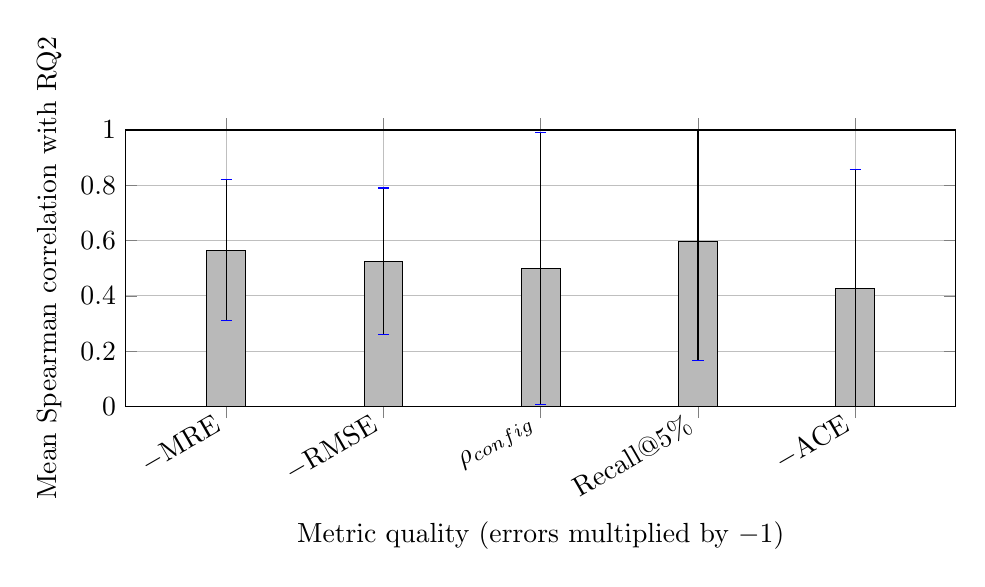
\begin{tikzpicture}
\begin{axis}[
    ybar,
    width=\linewidth,
    height=0.42\linewidth,
    ymin=0,
    ymax=1.0,
    ylabel={Mean Spearman correlation with RQ2},
    xlabel={Metric quality (errors multiplied by $-1$)},
    xtick={1, 2, 3, 4, 5},
    xticklabels={{$-$MRE}, {$-$RMSE}, {$\rho_{config}$}, {Recall@5\%}, {$-$ACE}},
    x tick label style={rotate=30, anchor=east},
    bar width=14pt,
    enlarge x limits=0.16,
    grid=major,
]
\addplot+[
    draw=black,
    fill=gray!55,
    error bars/y dir=both,
    error bars/y explicit,
] coordinates {
        (1,0.565) +- (0,0.255)
        (2,0.525) +- (0,0.265)
        (3,0.499) +- (0,0.493)
        (4,0.597) +- (0,0.431)
        (5,0.426) +- (0,0.431)
    };
\end{axis}
\end{tikzpicture}
